\documentclass{article}

% if you need to pass options to natbib, use, e.g.:
\PassOptionsToPackage{numbers, compress}{natbib}
% before loading neurips_2021

% ready for submission
%\usepackage{neurips_2021}

% to compile a preprint version, e.g., for submission to arXiv, add add the
% [preprint] option:
%     \usepackage[preprint]{neurips_2021}

% to compile a camera-ready version, add the [final] option, e.g.:
\usepackage[final]{neurips_2021}

% to avoid loading the natbib package, add option nonatbib:
%    \usepackage[nonatbib]{neurips_2021}

\usepackage[utf8]{inputenc} % allow utf-8 input
\usepackage[T1]{fontenc}    % use 8-bit T1 fonts
\usepackage[colorlinks=true,linkcolor=blue,urlcolor=blue,citecolor=purple]{hyperref}       % hyperlinks
\usepackage{url}            % simple URL typesetting
\usepackage{booktabs}       % professional-quality tables
\usepackage{amsfonts}       % blackboard math symbols
\usepackage{nicefrac}       % compact symbols for 1/2, etc.
\usepackage{microtype}      % microtypography
\usepackage{xcolor}         % colors
\usepackage{mathtools}
\usepackage{etoolbox}
\usepackage{amssymb}
\usepackage{bm}
\usepackage{float}
\usepackage{graphicx}

\usepackage{fullpage}

\input{~/Developer/Template/Academic/Math.tex}
\input{~/Developer/Template/Academic/ListStyle.tex}

\usepackage{import}
\usepackage{xifthen}
\usepackage{pdfpages}
\usepackage{transparent}
\newcommand{\incfig}[1]{%
	\def\svgwidth{\columnwidth}
	\import{./Figures/}{#1.pdf_tex}
}

% Appendix environment
\usepackage{appendix}
\def\sectionautorefname{Section}
\def\subsectionautorefname{Section}
\def\appendixautorefname{Appendix}
\renewcommand\appendixname{Appendix}
\renewcommand\appendixtocname{Appendix}
\renewcommand\appendixpagename{Appendix}
% begin appendix autoref patch [\autoref subsections in appendix](https://tex.stackexchange.com/questions/149807/autoref-subsections-in-appendix)
\makeatletter
\patchcmd{\hyper@makecurrent}{%
	\ifx\Hy@param\Hy@chapterstring
		\let\Hy@param\Hy@chapapp
	\fi}{%
	\iftoggle{inappendix}{%true-branch
		% list the names of all sectioning counters here
		\@checkappendixparam{chapter}%
		\@checkappendixparam{section}%
		\@checkappendixparam{subsection}%
		\@checkappendixparam{subsubsection}%
		\@checkappendixparam{paragraph}%
		\@checkappendixparam{subparagraph}%
	}{}%
}{}{\errmessage{failed to patch}}

\newcommand*{\@checkappendixparam}[1]{%
	\def\@checkappendixparamtmp{#1}%
	\ifx\Hy@param\@checkappendixparamtmp
		\let\Hy@param\Hy@appendixstring
	\fi
}
\makeatletter

\newtoggle{inappendix}
\togglefalse{inappendix}

\apptocmd{\appendix}{\toggletrue{inappendix}}{}{\errmessage{failed to patch}}
\apptocmd{\subappendices}{\toggletrue{inappendix}}{}{\errmessage{failed to patch}}
% end appendix autoref patch

\title{EECS 545 Machine Learning\\Progress Report\\GNN on Traveling Salesman Problem}

% The \author macro works with any number of authors. There are two commands
% used to separate the names and addresses of multiple authors: \And and \AND.
%
% Using \And between authors leaves it to LaTeX to determine where to break the
% lines. Using \AND forces a line break at that point. So, if LaTeX puts 3 of 4
% authors names on the first line, and the last on the second line, try using
% \AND instead of \And before the third author name.

\author{%
  Pingbang Hu\\
  Department of Computer Science\\
  University of Michigan\\
  \texttt{pbb@umich.edu} \\
  \And
  Jonathan Moore \\
  Department of Computer Science\\
  University of Michigan\\
  \texttt{moorejon@umich.edu} \\
  \And
  Yi Zhou \\
  Department of Math\\
  University of Michigan\\
  \texttt{yizho@umich.edu} \\
  \And
  Shubham Kumar Pandey \\
  Department of Statistics\\
  University of Michigan\\
  \texttt{pandeysk@umich.edu} \\
  \And
  Anuraag Ramesh \\
  Department of Statistics\\
  University of Michigan\\
  \texttt{anuraagr@umich.edu} \\
}


\begin{document}

\maketitle

\begin{abstract}
	%Yi Zhou

	This is our progress report for the EECS 545 course project. Graph neural network is a rising concept in computer science that has demonstrated significant potential in many areas. Our project aims to
	further demonstrate its potential by applying it to the classic traveling salesman problem. After generating the dataset, we will first use imitation learning to obtain a pretty good path, which will
	then be inputted into reinforcement learning to obtain the optimal solution. Since imitation learning converges very fast, we expect our run time to be promising, for larger datasets, compared to tradition exact solvers.

	In this progress report, we will describe and explain our proposed method, share important related works, show our difference with the existing works, present our experimental results, and set up weekly goals for future development.

	\paragraph{Keywords:} Travelling salesman problem, Graph Neural Network, Imitation Training, Reinforcement Learning, Transformer, Integer Programming, Embedding learning, Link Prediction, Combinatorial
	Optimization, Learning theory.
\end{abstract}


\section{Introduction}
%Yi Zhou

The travelling salesman problem, also called the travelling salesperson problem or TSP, is a problem as follows. Given a list of cities and the distances between each pair of cities, we want
to find the shortest possible route that visits each city \emph{exactly once} and returns to the origin city.

Specifically, given an \textbf{undirected weighted graph} \(\mathcal{G} = (\mathcal{E}, \mathcal{V})\), which is an ordered pair of nodes set \(\mathcal{E}\) and edges set
\(\mathcal{V}\subseteq \mathcal{E}\times\mathcal{E}\) where \(\mathcal{G}\) is equipped with \textbf{spatial structure}. This means that each edge between nodes will have different weights and each
node will have its coordinates, we want to find a simple cycle that visits every node exactly once while having the smallest cost.

Our approach is based on the application of graph neural networks. After generating the dataset, we will first use imitation learning to obtain a pretty good path, which will then be inputted into unsupervised
reinforcement learning to obtain the optimal solution. Since imitation learning converges very fast, we expect our run time to be promising, for large datasets, compared to tradition exact solvers.

\section{Proposed Method}
\subsection{Problem Formulation}
\subsubsection{TSP as Integer Linear Programming}
We first formulate TSP in terms of \textbf{Integer Linear Programming}. Given an undirected weighted group \(\mathcal{G} = (\mathcal{E}, \mathcal{V})\), we label the
nodes with numbers \(1, \ldots, n\) and define
\[
	x_{ij}\coloneqq \begin{dcases}
		1, & \text{if }(i, j)\in \mathcal{E}^\prime                       \\
		0, & \text{if } (i, j)\in \mathcal{E}\setminus\mathcal{E}^\prime,
	\end{dcases}
\]
where \(\mathcal{E}^\prime\subset \mathcal{E}\) is a variable which can be viewed as a compact representation of all variables \(x_{ij}\), \(\forall i, j\). Furthermore, we
denote the weight on edge \((i, j)\) by \(c_{ij}\), then for a particular TSP problem instance, we can formulate the problem as follows.
\begin{equation}\label{formula:TSP}
	\begin{aligned}
		\min & \sum _{i=1}^{n}\sum _{j\neq i,j=1}^{n}c_{ij}x_{ij}\colon &  &                      \\
		     & x_{ij}\in \{0,1\}                                        &  & i,j=1,\ldots ,n;     \\
		     & u_{i}\in \mathbb{Z}                                      &  & i=2,\ldots ,n;       \\
		     & \sum _{i=1,i\neq j}^{n}x_{ij}=1                          &  & j=1,\ldots ,n;       \\
		     & \sum _{j=1,j\neq i}^{n}x_{ij}=1                          &  & i=1,\ldots ,n;       \\
		     & u_{i}-u_{j}+nx_{ij}\leq n-1                              &  & 2\leq i\neq j\leq n; \\
		     & 1\leq u_{i}\leq n-1                                      &  & 2\leq i\leq n.
	\end{aligned}
\end{equation}

This is the Miller-Tucker-Zemlin formulation\cite{MTZ-formulation}. Note that in our case, since we're going to solve TSP exactly, hence all variables are integers,
and we sometimes call this kind of integer linear programming as \textbf{pure integer programming}.

Since integer programming is a NP-Hard problem, there are no known polynomial algorithm can solve this explicitly. Hence, modern approach to such a problem is to
\textbf{relax} the integrality constraint, which makes \autoref{formula:TSP} becomes a continuous linear programming (LP), whose solution provides a lower bound to
\autoref{formula:TSP} since it's a relaxation, and we're trying to find the minimum.

Since an LP is a convex optimization problem, we have many polynomial time algorithms to solve the relaxed version. After obtaining a relaxed solution, if such LP relaxed
solution respects the integrality constraint, we see that it's indeed a solution to \autoref{formula:TSP}. But if not, we can simply divide the original relaxed LP into two
sub-problems by \textbf{splitting the feasible region} according to a variable that does not respect integrality in the current relaxed LP solution \(\bm{x}^\ast\),
\begin{equation}\label{eq:branch-and-bound}
	x_{i} \leq \left\lfloor x_{i}^\ast \right\rfloor\lor x_{i} \geq \left\lceil x_{i}^\ast \right\rceil,\qquad \exists i\leq p\mid x_{i} ^\ast \notin \mathbb{\MakeUppercase{z}}.
\end{equation}

We see that by adding such additional constraint in two sub-problems respectively, we get a recursive algorithm called \textbf{Branch-and-Bound} \cite{B&B.ch7}.

\subsubsection{Branching Rules}
The branch-and-bound algorithm is widely used to solve integer programming problems. We see that the key step in the branch-and-bound algorithm is selecting a non-integer
variable to \underline{branch on} in \autoref{eq:branch-and-bound}. And as one can expect, some choices may reduce the recursive searching tree
significantly \cite{B&B.branching-impact}, hence the \emph{branching rules} are the core of modern combinatorial optimization solvers, and it has been the focus of extensive
research \cite{B&B-branching-rules-research-1, B&B-branching-rules-research-2, B&B-branching-rules-research-3, B&B-branching-rules-research-4}. There are several popular
strategies \cite{branching-rules-revisited} used in modern solver.
\begin{enumerate}
	\item Strong branching. It'll result in the smallest recursive tree by computing the expected bound improvement for \textbf{each} candidate variable before branching by
	      finding solutions of two LPs for every candidate, which is undoubtedly, very expensive. \cite{Finding-cuts-in-the-TSP}
	\item Hybrid branching. Which basically computes a strong branching scores only at the beginning of the solving, and gradually switches to other methods like
	      \underline{Conflict score}, \underline{Pseudo-cost} \cite{B&B-branching-rules-research-2}, or some hand-crafted combinations of above. \cite{branching-rules-revisited, B&B-branching-rules-research-4}.
\end{enumerate}

\subsection{Theoretical Framework}
Our objective is to learn branching strategy without expensive evaluation. And since this is a discrete time control process, hence we model the problem by Markov Decision Process (MDP) \cite{howard1960dynamic}.

\subsubsection{Markov Decision Process (MDP)}
Given a regular Markov decision process \(\mathcal{M} \coloneqq (\mathcal{S}, \mathcal{A}, p_{\mathrm{init}}, p_{\mathrm{trans}}, R)\), where we have
\begin{itemize}
	\item State space \(\mathcal{S}\)
	\item Action space \(\mathcal{A}\)
	\item Initial state distribution \(p_{\mathrm{init}}\colon \mathcal{S} \to \mathbb{R}_{\geq 0}\)
	\item State transition distribution \(p_{\mathrm{trans}}\colon \mathcal{S}\times \mathcal{A}\times \mathcal{S} \to \mathbb{R}_{\geq 0}\)
	\item Reward function \(R\colon \mathcal{S} \to \mathbb{R}\)
\end{itemize}

We note that in the above definition of Markov Decision Process, the reward function \(R\) need not be deterministic. In other words, we can define \(R\) as a random function
which will take a value based on a particular state in \(\mathcal{S}\) with some randomness. Note that if \(R\) in \(\mathcal{M}\) is equipped with any kind of randomness, we can
write the reward \(r_t\) at time \(t\) as
\[
	r_t\sim p_{\mathrm{reward}}(r_t\mid s_{t-1}, a_{t-1}, s_t),
\]
and this can be converted into an equivalent Markov Decision Process \(\mathcal{M}^\prime\) with a deterministic reward function \(R^\prime\), where the randomness is integrated
into parts of the states.

With an action policy \(\pi \colon \mathcal{A}\times \mathcal{S}\to \mathbb{R}_{\geq 0}\) such that the action \(a_t\) taken at time \(t\) is determined by
\[
	a_t\sim \pi(a_t\mid s_t),
\]
we see that an MDP can be unrolled to produce a \emph{trajectories} composed by state-action pairs as
\[
	\tau = (s_0, a_0, s_1, a_1, \ldots)
\]
which obeys the joint distribution
\[
	\tau \sim \underbrace{p_{\mathrm{init}}(s_0)}_{\text{initial state}}\prod_{t = 0}^{\infty} \underbrace{\pi(a_t\mid s_t)}_{\text{next action}}\underbrace{p_{\mathrm{trans}}(s_{t+1}\mid a_t, s_t)}_{\text{next state}}.
\]

\subsubsection{Partially Observable Markov Decision Process (PO-MDP)}
Follows the same idea from MDP, in the PO-MDP setting deals with the case that when the \textbf{complete} information about the current MDP state \(\mathcal{S}\) is unavailable
or not necessarily for the decision-making \cite{ASTROM1965174}. Instead, in our case, only a partial \textbf{observation} \(o\in \Omega\) is available, where \(\Omega\) is called the
\textbf{partial state space}. We can use an active perspective to view the above model, namely we're merely applying a \underline{observation function}
\(O\colon \mathcal{S}\to \Omega\) to the current state \(s_t\) at each time step \(t\).  Hence, we define a PO-MDP \(\widetilde{\mathcal{M}}\) as a tuple
\[
	\widetilde{\mathcal{M}} \coloneqq (\mathcal{S}, \mathcal{A}, p_{\mathrm{init}}, p_{\mathrm{trans}}, R, O).
\]

Within this setup, a trajectory of PO-MDP takes form as
\[
	\tau = (o_0, r_0, a_0, o_1, r_1, a_1, \ldots),
\]
where \(o_t\coloneqq O(s_t)\) and \(r_t\coloneqq R(s_t)\). Specifically, noting that here \(r_t\) still depends on the state of the OP-MDP, not the observation.

We introduce a convenience variable \(h_t\colon (o_0, r_0, a_0, \ldots, o_t, r_t)\in \mathcal{H}\), which represents the PO-MDP history at time step \(t\) \textbf{without the
	action} \(a_t\).  Due to the non-Markovian nature of the trajectories,
\[
	o_{t+1}, r_{t+1}\not\perp h_{t-1} \mid o_t,r_t,a_t,
\]
namely the decision-maker must take the whole history of observations, rewards and actions into account to decide on an optimal action at current time step \(t\). We then see
that action policy for PO-MDP takes the form
\(\widetilde{\pi}\colon \mathcal{A}\times \mathcal{H}\to \mathbb{R}_{\geq 0}\) such that \(a_t\sim \pi (a_t\mid h_t)\).

\subsection{Markov Control Problem}
We define the MDP control problem as that of finding a policy \(\pi ^\ast\colon \mathcal{A}\times \mathcal{S}\to \mathbb{R}_{\geq 0}\)
which is optimal with respect to the expected total reward, that is,
\[
	\pi^\ast = \underset{\pi}{\arg\max} \lim_{T\to \infty}\mathbb{E}_\tau\left[\sum_{t=0}^T r_t\right],
\]
where \(r_t\coloneqq R(s_t)\). To generalize this into PO-MDP control problem, similar to the MDP control problem, the objective is to find a policy
\(\widetilde{\pi}^\ast\colon \mathcal{A}\times \mathcal{H}\to \mathbb{R}_{\geq 0}\) such that it maximizes the expected total rewards. By slightly abusing the notation, we
simply denote this learned policy by \(\widetilde{\pi}^\ast\) where the objective function is completely the same as in the MDP case.

\subsection{Learning Pipeline}
Since the branch-and-bound variable selection problem can be naturally formulated as a Markov decision process, hence a natural machine learning algorithm to use is reinforcement learning \cite{sutton2018reinforcement}.
Specifically, since there are some state-of-the-art (SOTA) integers programming solvers out there, for examples, \texttt{Gurobi}\footnote{\url{https://www.gurobi.com/}}, \texttt{SCIP}\footnote{\url{https://www.scipopt.org/}}, etc,
we decide to try imitating learning\cite{Imitation-Learning-A-Survey-of-Learning-Methods} by learning directly from an expert branching rule.

While there are some related works in this approach \cite{GasseCFCL19} aiming to tackle \textbf{mixed integer linear programming} (MILP), which means there are only some variables have integrality constraints, while
other variables can be real numbers. But our approach tries to extend this further, we're focusing on TSP, which not only is a pure integer programming, and the variables value is bounded to be in \(\{0, 1\}\) only.
Except all these, since imitating learning can't outperform SOTA solver in its nature, hence though the work in \cite{GasseCFCL19} is interesting, but we still think we can do better by focusing on a particular domain (TSP
in this case) and try to formulate a problem specific reward function for TSP.

Hence, our proposed learning pipeline is as follows. Firstly, we only use imitating learning following \cite{GasseCFCL19} to obtain a good enough model, then we turn to unsupervised learning setup under the framework of
reinforcement learning, which should make the network learn some domain-specific property and help to boost the performance. The implementation summary can be found in
\autoref{subsec:general-pipeline}.

\begin{figure}[H]
	\centering
	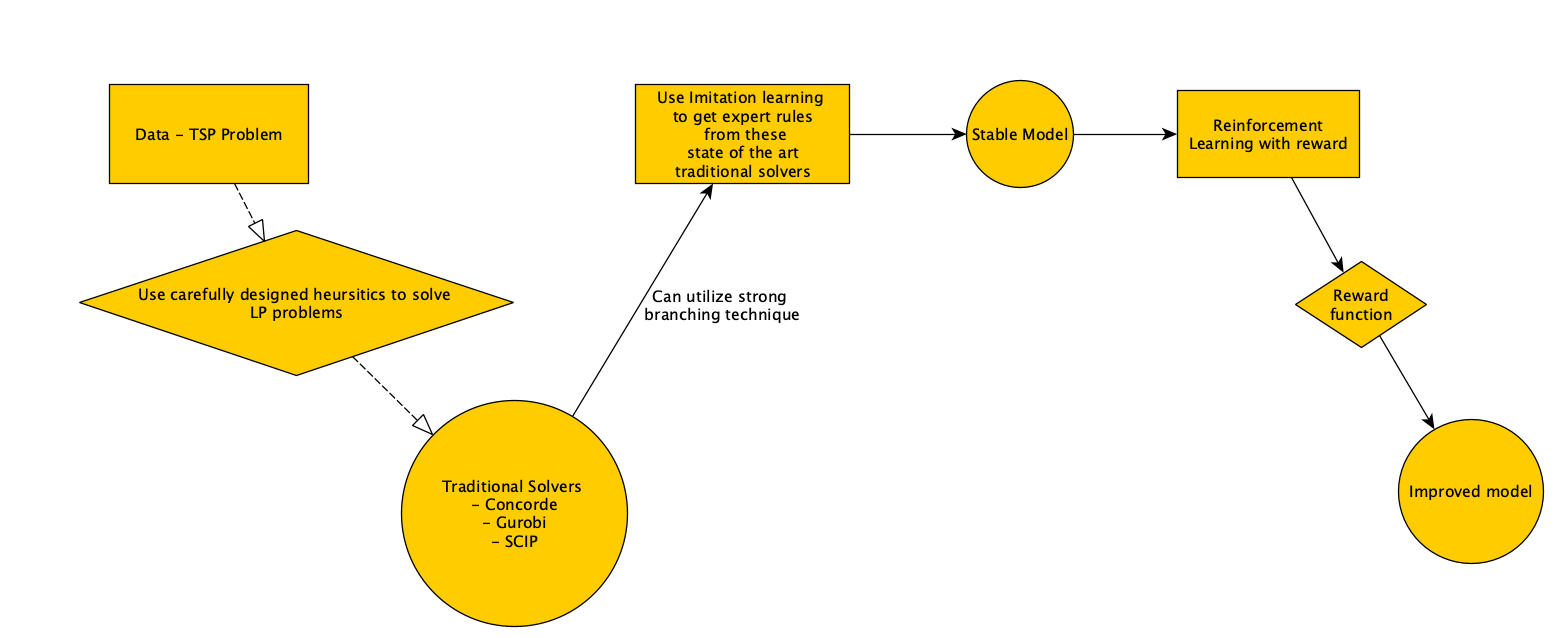
\includegraphics[width=\linewidth]{Figures/Pipeline.png}
	\caption{Implementation Pipeline}
\end{figure}

\subsubsection{Imitating Learning}
As we mentioned before, the most effective branching strategy is strong branching, hence we train the network by behavioral cloning \cite{Efficient-Training-of-artificial-Neural-Networks-for-Autonomous-Navigation}.
We first run the SOTA solver and get state-action pairs
\[
	\mathcal{\MakeUppercase{d}} = \left\{(s_{i} , \bm{a} _{i} ^\ast)\right\}_{i = 1}^N,
\]
and then learn our policy \(\widetilde{\pi} ^\ast\) b minimizing the cross-entropy loss
\[
	\mathcal{\MakeUppercase{l}} (\theta ) = - \frac{1}{N}\sum\limits_{(\bm{s}, \bm{a}^\ast)\in \mathcal{\MakeUppercase{d}} }\log \widetilde{\pi}_\theta (\bm{a} ^\ast \mid \bm{s} ).
\]

Additionally, we access (observe) the state of the branch-and-bound process by directly interacting with the SOTA solvers, specifically, \texttt{SCIP}. The implementation detail follows Gasse et al.\cite{GasseCFCL19}.

\subsubsection{Unsupervised Reinforcement Learning}
After getting a stable model, we remove the expert's instructions and let the model explore by itself since we're focusing on TSP, which is a particular problem type in pure integer programming. That is, we are now
going to define a new reward function \(R\colon \mathcal{\MakeUppercase{s}} \to \mathbb{\MakeUppercase{r}} \).

We are still exploring this part, but some useful and observable states can be used in our formulation of \(R\), including things like estimated branching tree sizes and its
decreasing rate, or current tour length and its decreasing rate, etc.

And also, we have some interesting idea about the objective of such reward function, like reward decay forcing fast solving, or providing additional information, like the
optimal tour length.

In this way, from the success in \cite{GasseCFCL19}, we're guaranteed with a good enough model status, namely a good enough branching strategy after our first stage. Then, we do not need to worry about the
technical detail in reinforcement learning like initial training but focus on giving a general pipeline for how to tackle a particular problem in this kind of combinatorial optimization problems.

Besides, there is a reason why we do not use pre-trained models from \cite{GasseCFCL19}. An obvious reason is that our focus is different: \cite{GasseCFCL19} focuses on general MILP, while we specifically focus on
TSP (Pure IP with bounded variable values), which is a slightly but still different field.\footnote{Using the pre-trained models will be a good idea to see the generalizability in RL after we obtain a good enough reward function.}

\section{Related Work}
%Jonathan Moore (Summarize the related papers)
Obviously, there has already been extensive work done to optimize TSP solvers both theoretically and practically. We have done extensive research into other solvers, the most important of which will be summarized.
\paragraph{Transformer Network for TSP \cite{Bresson2021TheTN}}
The main focus of this paper is to detail the application of deep reinforcement learning reapplied to a Transformer architecture originally created for NLP. Unlike our proposed model, this solver learns
heuristics with very low error rates (.004\% for 50 points and 0.39\% for 100 points) which can run over a TSP problem much faster than a traditional solver with similar results.

\paragraph{Exact Combinatorial Optimization with GCNNs \cite{GasseCFCL19}}
This paper serves as the one of the backbones of our research; its main focus is to detail how MIPS can potentially be solved much quicker than a traditional solver by using
GNNs (specifically GCNNs). It did this by training its model using imitation learning (using the strong branching expert rule) and was able to effectively produce outputs for
problem instance much greater than what they were trained on. By using this method in our own model, we can train using the ~1,000 node samples that traditional solvers can
compute quickly while still being able to solve several thousand node examples ourselves.
%Yi Zhou (state of the art exact solver; our difference with existing work.)

\paragraph{State of the Art Exact Solver}
There has been a lot of progress on the symmetric TSP in the last century. With the increase in the number of nodes, there is a
superpolynomial (at least exponential) explosion in the number of potential solutions. This makes the
TSP problem difficult to solve on two parameters, the first being finding a global shortest route as well as reducing the computation complexity in finding this route.
Concorde\footnote{\url{http://www.math.uwaterloo.ca/tsp/concorde/}}, written in the ANSI C programming language, is widely recognized as the state-of-the-art(fastest) exact TSP
solution for large datasets.

\paragraph{Our Difference With Existing Work}
Our approach to solve TSP exactly is different from the Concorde approach, as well as the methods mentioned in the papers above. We will first use imitation training, which has
been proven to converge fast, to obtain an approximation of the optimal path. Then, we will use our current path to initialize the reinforcement learning in order to obtain the global
shortest path. Our combination of the two methods on GNN might be a novel appraoch in solving TSP exactly. For problems with more than 1000 nodes, we
expect our approach to give promising run time compared to other existing exact solvers.

\section{Experimental Results}
%Pingbang Hu
Our implementation on the first part, imitating learning, is based on Ecole\footnote{\url{https://github.com/ds4dm/ecole}} and hugely follows the
work by Gasse et al.'\cite{GasseCFCL19} We now have a very simple implementation similar to the setup in the original paper, but with cleaner
API and code style.

%Jonathan Moore (Dataset and Pre-processing)
For our data, we will be using a data generator created from the Concorde TSP solver. This data generator will allow us to efficiently generate TSP problem sets of any size
that we want; additionally, we can use their solver as well in order to first generate our training set for imitation learning. Once we have moved out of imitation learning, it will still be
very useful to be able to have the ability to (relatively) quickly check our model's output for correctness.

Fortunately, as long as we design our model around the output of the Concorde TSP generator, we do not need any further pre-processing. The result is included in
\autoref{sec:sample-code-output}.

\section{Future Milestone}
\begin{enumerate}
	\item Define an explicit reward function.
	\item Using more sophisticated model in the imitating learning part.
	\item Benchmarking all results from different exact solver.
	\item Comparing the performance between using pre-trained model and not using one.
	\item Implement the code for TSP data generator and also all the learning algorithms.
	\item Give theoretical analysis of our result.
\end{enumerate}

%─────Conclusion────────────────────────────────────────────────────────────────────────────────────────────────────────────────────────────────────
\section{Conclusion}
We have done a comprehensive and detailed research about this topic, and decide to turn our focus on approximation algorithm to exact algorithm  for TSP
compare to what we have proposed at the beginning. We explored the potential of combinatorial optimization problem in machine learning and tried to
understand the previous works people have done. Additionally, we found the excellent library, Ecole, for the combinatorial optimization problem
in machine learning and tried to learn it in detail and integrate it into our implementation.

Besides all the exploration works, we also looked into the mathematical rigorous framework to model our problem, and give a quick overview of why
our methods should work based on the mathematical framework we gave. We are now ready to implement our proposed learning algorithm based on our current data generator moving forward.

%─────Author Contributions──────────────────────────────────────────────────────────────────────────────────────────────────────────────────────────
\section{Author Contributions}
All authors contributed equally to this work. Yi and Jonathan worked on drafting the abstract, introduction and related work. Pingbang and Shubham worked on the proposed method, finding rationale for why it should work, and intuition behind choosing this specific approach. Pingbang drafted the proposed method including the technical details. Anuraag and Pingbang worked on the implementation part, including getting familiar with the Ecole library. Anuraag worked on instance and data set generation and running initial steps on this library. Jonathan drafted the data set generation and experimental results.

\newpage
%─────Reference──────────────────────────────────────────────────────────────────────────────────────────────────────────────────────────────────────
\bibliographystyle{plainnat}
\bibliography{ref}

\newpage
%─────Appendix───────────────────────────────────────────────────────────────────────────────────────────────────────────────────────────────────────
\appendix
\appendixpage

\section{Sample Code Output}\label{sec:sample-code-output}
\subsection{General Pipeline}\label{subsec:general-pipeline}
Our code will include
\begin{itemize}
	\item \texttt{01\_generate\_instances.py}.
	\item \texttt{02\_generate\_dataset.py}.
	\item \texttt{03\_train\_gnn.py}.
	\item \texttt{04\_evaluate.py}.
\end{itemize}
We report the result of \texttt{01\_generate\_instances.py} and \texttt{02\_generate\_dataset.py} and leave the output for \texttt{03\_train\_gnn.py} and
\texttt{04\_evaluate.py} to the next time.

The overall pipeline should be summarized to the following simple script.
\begin{lstlisting}[language=commandline]
# Generate MILP instances
python 01_generate_instances.py TSP

# Generate supervised learning datasets
python 02_generate_dataset.py TSP -j 4  # number of available CPUs

# Training
for i in {0..4}
do
    python 03_train_gnn.py TSP -s $i
done

# Evaluation
python 04_evaluate.py TSP
\end{lstlisting}

\subsection{Data Generation}\label{subsec:data-generation-code}
In this section, we report some sample output after running our implementation for problem instances generator. Specifically, we implement a dataset
generator which will do the followings in sequence.
\begin{enumerate}
	\item \texttt{01\_generate\_instances.py}. This will essentially do
	      \begin{enumerate}
		      \item Generate instances of problem randomly by the number we specify.
		      \item Pass the generated problem instances to \texttt{SCIP} and record all the observation from \texttt{SCIP} during the solving.
	      \end{enumerate}
	\item \texttt{02\_generate\_dataset.py}. This will essentially do
	      \begin{enumerate}
		      \item Wrap problem instances and also the corresponding observations into one big dataset to use later.
	      \end{enumerate}
\end{enumerate}
\subsubsection{Instance Generation}
After utilizing the Ecole library, we have tried to generate some sample problem instances for \texttt{setcover}. Here is the result.
\begin{lstlisting}[style=DOS]
1000 instances in data/instances/setcover/train_500r_1000c_0.05d
200 instances in data/instances/setcover/valid_500r_1000c_0.05d
10 instances in data/instances/setcover/transfer_50r_1000c_0.05d
10 instances in data/instances/setcover/transfer_100r_1000c_0.05d
10 instances in data/instances/setcover/transfer_200r_1000c_0.05d
200 instances in data/instances/setcover/test_50r_100c_0.05d
  generating file data/instances/setcover/train_500r_1000c_0.05d/instance_1.lp ...
  generating file data/instances/setcover/train_500r_1000c_0.05d/instance_2.lp ...
  generating file data/instances/setcover/train_500r_1000c_0.05d/instance_3.lp ...
  ...
  generating file data/instances/setcover/train_500r_1000c_0.05d/instance_999.lp ...
  generating file data/instances/setcover/train_500r_1000c_0.05d/instance_1000.lp ...
  generating file data/instances/setcover/valid_500r_1000c_0.05d/instance_1.lp ...
  generating file data/instances/setcover/valid_500r_1000c_0.05d/instance_2.lp ...
  generating file data/instances/setcover/valid_500r_1000c_0.05d/instance_3.lp ...
  ...
  generating file data/instances/setcover/valid_500r_1000c_0.05d/instance_199.lp ...
  generating file data/instances/setcover/valid_500r_1000c_0.05d/instance_200.lp ...
  generating file data/instances/setcover/transfer_50r_1000c_0.05d/instance_1.lp ...
  generating file data/instances/setcover/transfer_50r_1000c_0.05d/instance_2.lp ...
  generating file data/instances/setcover/transfer_50r_1000c_0.05d/instance_3.lp ...
  ...
  generating file data/instances/setcover/transfer_50r_1000c_0.05d/instance_9.lp ...
  generating file data/instances/setcover/transfer_50r_1000c_0.05d/instance_10.lp ...
  generating file data/instances/setcover/transfer_100r_1000c_0.05d/instance_1.lp ...
  generating file data/instances/setcover/transfer_100r_1000c_0.05d/instance_2.lp ...
  generating file data/instances/setcover/transfer_100r_1000c_0.05d/instance_3.lp ...
  ...
  generating file data/instances/setcover/transfer_100r_1000c_0.05d/instance_9.lp ...
  generating file data/instances/setcover/transfer_100r_1000c_0.05d/instance_10.lp ...
  generating file data/instances/setcover/transfer_200r_1000c_0.05d/instance_1.lp ...
  generating file data/instances/setcover/transfer_200r_1000c_0.05d/instance_2.lp ...
  generating file data/instances/setcover/transfer_200r_1000c_0.05d/instance_3.lp ...
  ...
  generating file data/instances/setcover/transfer_200r_1000c_0.05d/instance_9.lp ...
  generating file data/instances/setcover/transfer_200r_1000c_0.05d/instance_10.lp ...
  generating file data/instances/setcover/test_50r_100c_0.05d/instance_1.lp ...
  generating file data/instances/setcover/test_50r_100c_0.05d/instance_2.lp ...
  generating file data/instances/setcover/test_50r_100c_0.05d/instance_3.lp ...
  ...
  generating file data/instances/setcover/test_50r_100c_0.05d/instance_199.lp ...
  generating file data/instances/setcover/test_50r_100c_0.05d/instance_200.lp ...
done.
\end{lstlisting}

\subsubsection{Dataset Generation}
Also, we have implement the code template which split the data into training set, validation and also testing set and wrapped them up.
Here is the output.
\begin{lstlisting}[style=DOS]
seed 0
1000 train instances for 1000 samples
200 validation instances for 200 samples
0 test instances for 200 samples
[w Thread-2] episode 0, seed 3789440165, processing instance 'data/instances/setcover/train_500r_1000c_0.05d/instance_154.lp'...
[w Thread-3] episode 1, seed 3998999672, processing instance 'data/instances/setcover/train_500r_1000c_0.05d/instance_651.lp'...
[w Thread-4] episode 2, seed 3665041058, processing instance 'data/instances/setcover/train_500r_1000c_0.05d/instance_364.lp'...
[w Thread-5] episode 3, seed 2122579412, processing instance 'data/instances/setcover/train_500r_1000c_0.05d/instance_829.lp'...
[w Thread-4] episode 2 done, 3 samples
[w Thread-4] episode 4, seed 92199959, processing instance 'data/instances/setcover/train_500r_1000c_0.05d/instance_706.lp'...
[m MainThread] 1 / 1000 samples written, ep 0 (4 in buffer).
[m MainThread] 2 / 1000 samples written, ep 0 (4 in buffer).
[m MainThread] 3 / 1000 samples written, ep 0 (4 in buffer).
...
[m MainThread] 111 / 1000 samples written, ep 0 (226 in buffer).
[m MainThread] 112 / 1000 samples written, ep 0 (231 in buffer).
[m MainThread] 113 / 1000 samples written, ep 0 (233 in buffer).
[w Thread-2] episode 0 done, 113 samples
[w Thread-2] episode 5, seed 3084161443, processing instance 'data/instances/setcover/train_500r_1000c_0.05d/instance_492.lp'...
...
[m MainThread] 999 / 1000 samples written, ep 1 (2899 in buffer).
[m MainThread] 1000 / 1000 samples written, ep 1 (2901 in buffer).
[w Thread-7] episode 0, seed 4086331612, processing instance 'data/instances/setcover/valid_500r_1000c_0.05d/instance_116.lp'...
[w Thread-8] episode 1, seed 4177056010, processing instance 'data/instances/setcover/valid_500r_1000c_0.05d/instance_34.lp'...
[w Thread-9] episode 2, seed 1004525138, processing instance 'data/instances/setcover/valid_500r_1000c_0.05d/instance_36.lp'...
[w Thread-10] episode 3, seed 2483450156, processing instance 'data/instances/setcover/valid_500r_1000c_0.05d/instance_14.lp'...
[w Thread-4] episode 14 done, 1078 samples
[m MainThread] 1 / 200 samples written, ep 0 (5 in buffer).
[m MainThread] 2 / 200 samples written, ep 0 (8 in buffer).
[m MainThread] 3 / 200 samples written, ep 0 (12 in buffer).
...
\end{lstlisting}

% \subsection{Training}\label{sbusec:traing-code}
% \subsubsection{Imitation Learning}\label{subsec:imitation-learning-code}

% \subsubsection{Reinforcement Learning}\label{subsec:reinforcement-learning-code}

% \subsection{Evaluation}\label{subsec:evaluation-code}

\end{document}